\documentclass[11pt]{article}

% if you need to pass options to natbib, use, e.g.:
%\PassOptionsToPackage{numbers}{natbib}
\usepackage[colorlinks,linkcolor=blue,filecolor=blue,citecolor=magenta,urlcolor=blue]{hyperref}
\usepackage{bm,amsmath,amsthm,amssymb,multicol,algorithmic,algorithm,enumitem,graphicx,subfigure}
\usepackage{xargs}
\usepackage{stmaryrd}
\usepackage{natbib}

% ready for submission
\usepackage{neurips_2020}
\def\M{\mathcal{M}}
\def\A{\mathcal{A}}
\def\Z{\mathcal{Z}}
\def\S{\mathcal{S}}
\def\D{\mathcal{D}}
\def\R{\mathcal{R}}
\def\P{\mathcal{P}}
\def\K{\mathcal{K}}
\def\E{\mathbb{E}}
\def\F{\mathfrak{F}}
\def\l{\boldsymbol{\ell}}

\newtheorem{Fact}{Fact}
\newtheorem{Lemma}{Lemma}
\newtheorem{Prop}{Proposition}
\newtheorem{Theorem}{Theorem} 
\newtheorem{Def}{Definition}
\newtheorem{Corollary}{Corollary}
\newtheorem{Conjecture}{Conjecture}
\newtheorem{Property}{Property}
\newtheorem{Observation}{Observation}
\newtheorem{Exa}{Example}
\newtheorem{assumption}{H\!\!}
\newtheorem{Remark}{Remark}
\newtheorem*{Lemma*}{Lemma}
\newtheorem*{Theorem*}{Theorem}
\newtheorem*{Corollary*}{Corollary}
 
\newcommand{\eqsp}{\;}
\newcommand{\beq}{\begin{equation}}
\newcommand{\eeq}{\end{equation}}
\newcommand{\eqdef}{\mathrel{\mathop:}=}
\def\EE{\mathbb{E}}
\newcommand{\norm}[1]{\left\Vert #1 \right\Vert}
\newcommand{\pscal}[2]{\left\langle#1\,|\,#2 \right\rangle}
\def\major{\mathsf{M}}
\def\rset{\ensuremath{\mathbb{R}}}

\begin{document}
\title{Sparsified Distributed Adaptive Learning with Error Feedback}

\author{
Xiaoyun Li \\
  Cognitive And Computing Lab\\
  Baidu Research\\
  Beijing, USA \\
  \texttt{xiaoyun@baidu.com} 
   \And
  Belhal Karimi \\
  Cognitive And Computing Lab\\
  Baidu Research\\
  Beijing, China \\
  \texttt{v_karimibelhal@baidu.com} 
   \And
  Ping Li \\
  Cognitive And Computing Lab\\
  Baidu Research\\
  Beijing, China \\
  \texttt{liping@baidu.com} \\
}

\date{\today}

\maketitle

\begin{abstract}
To be completed...
\end{abstract}

\section{Introduction}\label{sec:introduction}

Most modern machine learning tasks can be casted as a large finite-sum optimization problem written as:
\begin{equation}\label{eq:opt}
\min \limits_{\theta \in \Theta} \frac{1}{n} \sum_{i=1}^n f_i(\theta)
\end{equation}
where $n$ denotes the number of workers, $f_i$ represents the average loss for worker $i$ and $\theta$ the global model parameter taking value in $\Theta$, a subset of $\mathbb{R}^d$.



Some related work:


\citep{karimireddy2019error} develops variant of signSGD (as a biased compression schemes) for distributed optimization. Contributions are mainly on this error feedback variant.
In \citep{shi2019convergence}, the authors provide theoretical results on the convergence of sparse Gradient SGD for distributed optimization (we want that for AMS here).
\citep{stich2018sparsified} develops a variant of distributed SGD with sparse gradients too. Contributions include a memory term used while compressing the gradient (using top k for instance). Speeding up the convergence in $\frac{1}{T^3}$.
% \url{https://arxiv.org/pdf/1901.09847.pdf}
% \url{https://pdfs.semanticscholar.org/8728/dee89906022c1d4f5c1de1233c3f65ab92f2.pdf?_ga=2.152244026.2027005181.1606271153-15127215.1603945483}
% \url{https://proceedings.neurips.cc/paper/2018/file/b440509a0106086a67bc2ea9df0a1dab-Paper.pdf}


\section{Preliminaries}\label{sec:prelim}

\paragraph{Sparse Optimization Methods. } 


\paragraph{Distributed Learning. }
When a large number of compute engines is available, being able to train global machine learning models while mutualizing the available and \emph{decentralized} source of computation has been a growing focus for the community.

Decentralized optimization methods include methods such as ADMM~\citep{boyd2011distributed}, Distributed Subgradient Descent~\citep{nedic2009distributed}, Dual Averaging~\citep{duchi2011dual}, Prox-PDA~\citep{hong2017prox}, GNSD~\citep{lu2019gnsd}, and Choco-SGD~\citep{koloskova2019decentralized}.  

A recent work \citep{chen2020quantized}, which focuses on adaptive gradient methods, namely the Adam \citep{kingma2014adam} annd the  AMSGrad~\citep{reddi2019convergence} optimization methods, develops a decentralized variant of gradient based and adaptive methods in the context of gossip protocols.
To date, very few contributions provided attempt to efficiently run adaptive gradient method is such a distributed setting.
Apart from \citep{chen2020quantized}, \citet{nazari2019dadam} proposes a decentralized version of AMSGrad~\citep{reddi2019convergence} which provably satisfies some non-standard regret.
Though, no sparsified variants of them have been proposed for practical purposes nor been studied in the literature.

\paragraph{Compression-Based Distributed Optimization. }
While the capabilities of the compute powers is exploding, the communication complexity between either the central server and the decentralized workers or among workers is becoming ineffectively large~\citep{chilimbi2014project, mcmahan2017communication}. 
Gradient sparsification constitutes one popular method to induce sparsity through the optimization procedure and reduce the number of bits transmitted at each iteration.
Extensive works have studied this technique to improve the communication efficiency of SGD-based methods such as distributed SGD.
This large class of sparsification techniques include gradient quantization leveraging quantized vector of gradients in the communication phase \citep{alistarh2017qsgd,wen2017terngrad,jiang2018linear,wangni2017gradient,haddadpour2019trading,chen2010approximate,jegou2010product}, gradient sparsificaiton generally selection top k components of the vector to be communicated, see \citep{stich2018sparsified,aji2017sparse}, or variants of the particular SGD algorithm such as low-precision SGD \citep{bernstein2018signsgd,karimireddy2019error} proposing a trade-off between communication cost and precision, and signSGD \citep{de2017understanding,yang2019swalp} where only the signs of the gradient vectors are communicated.
Most of these works apply to the SGD method \citep{bottou2008} as a prototype where a novel method and some convergence results are presented with a rate of $\mathcal{O}(\frac{1}{\sqrt{T}})$ where $T$ denotes the total number of iterations, see \citep{alistarh2018convergence}, thus achieving the same rate as plain SGD, see \citep{ghadimi2013stochastic,karimi2019non}.

Yet these communication reduction techniques, still presents a negative dependence on the number of workers, typically a linear dependence.
Hence the need for even more efficient techniques which constitutes the object of our paper.




\section{Method}\label{sec:main}

Consider standard synchronous distributed optimization setting. AMSGrad is used as the prototype, and the local workers is only in charge of gradient computation.


\subsection{TopK AMSGrad with Error Feedback}




The key difference (and interesting part) of our TopK AMSGrad compared with the following arxiv paper ``Quantized Adam''\url{https://arxiv.org/pdf/2004.14180.pdf} is that, in our model only gradients are transmitted. In ``QAdam'', each local worker keeps a local copy of moment estimator $m$ and $v$, and compresses and transmits $m/v$ as a whole. Thus, that method is very much like the sparsified distributed SGD, except that $g$ is changed into $m/v$. In our model, the moment estimates $m$ and $v$ are computed only at the central server, with the compressed gradients instead of the full gradient. This would be the key (and difficulty) in convergence analysis.


\begin{algorithm}[H]
\caption{\algo\ for Distributed Learning} \label{alg:sparsams}
\begin{algorithmic}[1]

\STATE \textbf{Input}: parameter $\beta_1$, $\beta_2$, learning rate $\eta_t$. 
\STATE Initialize: central server parameter $\theta_{0} \in \Theta \subseteq \mathbb R^d$; $e_{t,i}=0$ the error accumulator for each worker; sparsity parameter $k$; $N$ local workers; $m_0=0$, $v_0=0$, $\hat v_0=0$

\FOR{$t=1$ to $T$}

\STATE\textbf{parallel for worker $i \in [n]$ do}:
\STATE\quad  Receive model parameter $\theta_{t}$ from central server
\STATE\quad  Compute stochastic gradient $g_{t,i}$ at $\theta_t$
\STATE\quad  Compute $\tilde g_{t,i}=TopK(g_{t,i}+e_{t,i},k)$ \label{line:topk}
\STATE\quad  Update the error $e_{t+1,i}=e_{t,i}+g_{t,i}-\tilde g_{t,i}$
\STATE\quad  Send $\tilde g_{t,i}$ back to central server
\STATE \textbf{end parallel}

\STATE \textbf{Central server do:}
\STATE $\bar g_{t}=\frac{1}{N}\sum_{i=1}^N \tilde g_{t,i}$
\STATE $m_t=\beta_1 m_{t-1}+(1-\beta_1)\bar g_t$
\STATE $v_t=\beta_2 v_{t-1}+(1-\beta_2)\bar g_t^2$
\STATE $\hat v_t=\max(v_t,\hat v_{t-1})$ \label{line:v}
\STATE Update global model $\theta_t=\theta_{t-1}-\eta_t\frac{m_t}{\sqrt{\hat v_t+\epsilon}}$

\ENDFOR
\end{algorithmic}
\end{algorithm}


\subsection{Convergence Analysis}

Several mild assumptions to make: Nonconvex and smooth loss function, unbiased stochastic gradient, bounded variance of the gradient, bounded norm of the gradient, control of the distance between the true gradient and its sparse variant.

Check \citep{chen2020quantized} starting with single machine  and extending to distributed settings (several machines).


Under the distributed setting, the goal is to derive an upper bound to the second order moment of the gradient of the objective function at some iteration $T_f \in [1, T]$.

\subsection{Mild Assumptions}
We begin by making the following assumptions.

\begin{assumption}\label{ass:smooth}(Smoothness)
For $i \in \inter$, $f_i$ is  L-smooth: $\norm{\nabla f_i (\theta) - \nabla f_i (\vartheta)} \leq L \norm{\theta-\vartheta}$.
\end{assumption}

\begin{assumption}\label{ass:boundgrad}(Unbiased and Bounded gradient \textbf{per worker})
For any iteration index $t >0$ and worker index $i \in \inter$, the stochastic gradient is unbiased and bounded from above: $\EE[g_{t,i}] = \nabla f_i(\theta_t)$ and $\norm{g_{t,i}} \leq G_i$.
\end{assumption}

\begin{assumption}\label{ass:quant}(Bounded variance \textbf{per worker})
For any iteration index $t >0$ and worker index $i \in \inter$, the variance of the noisy gradient is bounded: $\EE[|g_{t,i} - \nabla f_i(\theta_t)|^2] < \sigma_i^2$.
\end{assumption}

Denote by $Q(\cdot)$ the quantization operator Line~\ref{line:topk} of Algorithm~\ref{alg:sparsams}, which takes as input a gradient vector and returns a quantized version of it, and note $\tilde{g} \eqdef Q(g)$.
Assume that
\begin{assumption}\label{ass:var}(Bounded Quantization)
For any iteration $t >0$, there exists a constant $q >0$ such that $\norm{g_t - \tilde{g}_t} \leq q \norm{g_t}$, where $g_t$ is the stochastic gradient computed at iteration $t$.
\end{assumption}


Denote for all $\theta \in \Theta$:
\begin{equation}\label{eq:obj}
f(\theta) \eqdef  \frac{1}{n} \sum_{i=1}^n f_i(\theta) \, ,
\end{equation} 
where $n$ denotes the number of workers.



\subsection{Intermediary Lemmas}

\begin{Lemma}
Under Assumption\ref{ass:smooth} to Assumption\ref{ass:var}, with a decreasing sequence of stepsize $\{\eta_t\}_{t>0}$, we have:

\begin{equation}
\EE[\pscal{\nabla f(\theta_t)}{(\hat{V}_{t+1} + \epsilon \mathsf{I_d})^{-1/2} \bar{g}_t}] \leq \textcolor{red}{TBD}
\end{equation}
where $ \mathsf{I_d}$ is the identity matrix, $\hat{V_t}$ the diagonal matrix which diagonal entries are $\hat v_t=\max(v_t,\hat v_{t-1})$ defined Line~\ref{line:v} of Algorithm~\ref{alg:sparsams} and $\bar{g}_t$ is the aggregation of all \textbf{quantized} gradients from the workers.
\end{Lemma}



\begin{proof}
Decompose $\bar{g}_t$  as the unbiased stochastic gradients and quantized versions.
\end{proof}


\begin{Lemma}
Under Assumption\ref{ass:smooth} to Assumption\ref{ass:var}, with a decreasing sequence of stepsize $\{\eta_t\}_{t>0}$, we have:

\begin{equation}
\begin{split}
\EE[f(\theta_{t+1}) - f(\theta_{t}) ] \leq & \textcolor{red}{bound of Lemma1}- \eta_{t+1} \beta_1\EE[\pscal{\nabla f(\theta_t)}{(\hat{V}_{t} + \epsilon \mathsf{I_d})^{-1/2} m_{t}}]\\
& +  \left(\frac{L}{2} + \beta_1 L \right) \norm{\theta_t - \theta_{t}}^2\\
&+   \eta_{t+1} G^2 \EE[\sum_{j=1}^d \left[(\hat{v}^j_{t+1} + \epsilon )^{-1/2} - (\hat{v}^j_{t} + \epsilon )^{-1/2}  \right] ]
\end{split}
\end{equation}
where $d$ denotes the dimension of the parameter vector
\end{Lemma}



\begin{proof}


We first define multiple auxiliary sequences. For the first moment, define

\begin{align*}
    &\bar m_t=m_t+\mathcal E_t,\\   
    &\mathcal E_t=\beta_1\mathcal E_{t-1}+(1-\beta_1)(e_{t+1}-e_t),
\end{align*}
such that 
\begin{align*} 
    \bar m_t&=\bar m_t+\mathcal E_t\\
    &=\beta_1(m_t+\mathcal E_t)+(1-\beta_1)(\bar g_t+e_{t+1}-e_1)\\
    &=\beta_1\bar m_{t-1}+(1-\beta_1)g_t.
\end{align*}


Denote the following auxiliary variables at iteration $t+1$
\begin{align}
z_{t+1} = \theta_{t+1} + \frac{\beta_1}{1-\beta_1}(\theta_{t+1} - \theta_{t})
\end{align}

By assumption Assumption~\ref{ass:smooth}, we can write the smoothness condition on the overall objective \eqref{eq:obj}, between iteration $t$ and $t+1$:

\begin{equation}
f(\theta_{t+1}) \leq f(\theta_{t})+  \pscal{\nabla f(\theta_t)}{\theta_{t+1} - \theta_{t}} + \frac{L}{2} \norm{\theta_{t+1} - \theta_{t}}
\end{equation}

Denote by $\hat{V_t}$ the diagonal matrix which diagonal entries are $\hat v_t=\max(v_t,\hat v_{t-1})$ defined Line~\ref{line:v} of Algorithm~\ref{alg:sparsams}.
Hence, we obtain,
\begin{equation}
f(\theta_{t+1}) \leq f(\theta_{t}) - \eta_{t+1} \pscal{\nabla f(\theta_t)}{(\hat{V}_{t+1} + \epsilon \mathsf{I_d})^{-1/2} m_{t+1}} + \frac{L}{2} \norm{\theta_{t+1} - \theta_{t}}
\end{equation}
where $\mathsf{I_d}$ denotes the identity matrix.

We now take the expectation of those various terms conditioned on the filtration $\mathcal{F}_t$ of the total randomness up to iteration $t$.
\begin{equation}\label{eq:smooth1}
\EE[f(\theta_{t+1}) - f(\theta_{t}) ] \leq - \eta_{t+1} \EE[\pscal{\nabla f(\theta_t)}{(\hat{V}_{t+1} + \epsilon \mathsf{I_d})^{-1/2} m_{t+1}}] + \frac{L}{2} \EE[\norm{\theta_{t+1} - \theta_{t}}^2]
\end{equation}

We now focus on the computation of the inner product obtained in the equation above.
We have
\begin{align}
& \eta_{t+1}\EE[ \pscal{\nabla f(\theta_t)}{(\hat{V}_{t+1} + \epsilon \mathsf{I_d})^{-1/2} m_{t+1}}]  \label{innerprod}\\
  = &\eta_{t+1} \EE[\pscal{\nabla f(\theta_t)}{(\hat{V}_{t+1} + \epsilon \mathsf{I_d})^{-1/2} m_{t+1} + (\hat{V}_{t} + \epsilon \mathsf{I_d})^{-1/2} m_{t+1} - (\hat{V}_{t} + \epsilon \mathsf{I_d})^{-1/2} m_{t+1}} ]\notag\\
    = & \eta_{t+1}\EE[ \pscal{\nabla f(\theta_t)}{(\hat{V}_{t} + \epsilon \mathsf{I_d})^{-1/2} m_{t+1}} ] +  \eta_{t+1} \EE[\pscal{\nabla f(\theta_t)}{\left[(\hat{V}_{t+1} + \epsilon \mathsf{I_d})^{-1/2} - (\hat{V}_{t} + \epsilon \mathsf{I_d})^{-1/2}  \right]m_{t+1}}]\notag\\
 = & \eta_{t+1}\beta_1\EE[ \pscal{\nabla f(\theta_t)}{(\hat{V}_{t} + \epsilon \mathsf{I_d})^{-1/2} m_{t}}] +  \eta_{t+1} (1-\beta_1) \EE[\pscal{\nabla f(\theta_t)}{(\hat{V}_{t+1} + \epsilon \mathsf{I_d})^{-1/2} \bar{g}_t}] \notag\\
&+  \eta_{t+1} \EE[\pscal{\nabla f(\theta_t)}{\left[(\hat{V}_{t+1} + \epsilon \mathsf{I_d})^{-1/2} - (\hat{V}_{t} + \epsilon \mathsf{I_d})^{-1/2}  \right]m_{t+1}}] \label{decomp}
\end{align}
where $\bar{g}_t$ is the aggregated gradients from all workers.

Plugging the above in \eqref{eq:smooth1} yields:
\begin{equation}\label{eq:main1}
\begin{split}
&\EE[f(\theta_{t+1}) - f(\theta_{t}) ] \\
\leq & \underbrace{- \beta_1\EE[ \pscal{\nabla f(\theta_t)}{(\hat{V}_{t} + \epsilon \mathsf{I_d})^{-1/2} m_{t}}]}_{A_t} \eta_{t+1}\\
& \underbrace{-  \EE[\pscal{\nabla f(\theta_t)}{\left[(\hat{V}_{t+1} + \epsilon \mathsf{I_d})^{-1/2} - (\hat{V}_{t} + \epsilon \mathsf{I_d})^{-1/2}  \right]m_{t+1}}]}_{B_t}\eta_{t+1}\\
& \underbrace{-  (1-\beta_1) \EE[\pscal{\nabla f(\theta_t)}{(\hat{V}_{t+1} + \epsilon \mathsf{I_d})^{-1/2} \bar{g}_t}]}_{C_t} \eta_{t+1}+ \frac{L}{2} \EE[\norm{\theta_{t+1} - \theta_{t}}^2]
\end{split}
\end{equation}
To begin with, by the tower rule, we have that 
\begin{align}
A_t & = - \beta_1\EE[\EE[\pscal{\nabla f(\theta_t)}{(\hat{V}_{t} + \epsilon \mathsf{I_d})^{-1/2} m_{t}}| \mathcal{F}_t]] \\
& = - \beta_1 \pscal{\nabla f(\theta_{t-1})}{(\hat{V}_{t} + \epsilon \mathsf{I_d})^{-1/2} m_{t}}] - \beta_1 \pscal{\nabla f(\theta_t) - \nabla f(\theta_{t-1})}{(\hat{V}_{t} + \epsilon \mathsf{I_d})^{-1/2} m_{t}}]\\
\end{align}
where we recognize the first term as the term in \eqref{innerprod}, at iteration $t-1$ and hence apply the same decomposition as in \eqref{decomp}.
Coupling with the smoothness of $f$, which gives that
$$
- \beta_1 \pscal{\nabla f(\theta_t) - \nabla f(\theta_{t-1})}{(\hat{V}_{t} + \epsilon \mathsf{I_d})^{-1/2} m_{t}}] \leq \frac{\beta_1 L}{\eta_{t-1}} \norm{\theta_t - \theta_{t}}^2
$$

we obtain,
\begin{align}
A_t & = - \beta_1\EE[\EE[\pscal{\nabla f(\theta_t)}{(\hat{V}_{t} + \epsilon \mathsf{I_d})^{-1/2} m_{t}}| \mathcal{F}_t]]\\
&  \leq \eta_{t+1} \beta_1(A_{t-1} + B_{t-1} + C_{t-1})  + \eta_{t+1}\frac{\beta_1 L}{\eta_{t-1}} \norm{\theta_t - \theta_{t}}^2
\end{align}
Then,
\begin{align}
B_t & =-  \EE[\pscal{\nabla f(\theta_t)}{\left[(\hat{V}_{t+1} + \epsilon \mathsf{I_d})^{-1/2} - (\hat{V}_{t} + \epsilon \mathsf{I_d})^{-1/2}  \right]m_{t+1}}]\\
& =  \EE[\sum_{j=1}^d  \nabla^j f(\theta_t)m_{t=1}^j \left[(\hat{v}^j_{t+1} + \epsilon )^{-1/2} - (\hat{v}^j_{t} + \epsilon )^{-1/2}  \right] ]\\
& \overset{(a)}{\leq}  \EE[\norm{\nabla f(\theta_t)} \norm{m_{t=1}}\sum_{j=1}^d\left[(\hat{v}^j_{t+1} + \epsilon )^{-1/2} - (\hat{v}^j_{t} + \epsilon )^{-1/2}  \right] ]\\
& \overset{(b)}{\leq}  G^2 \EE[\sum_{j=1}^d \left[(\hat{v}^j_{t+1} + \epsilon )^{-1/2} - (\hat{v}^j_{t} + \epsilon )^{-1/2}  \right] ]
\end{align}
where $\nabla^j f(\theta_t)$ denotes the j-th component of the gradient vector $\nabla f(\theta_t)$, (a) uses of the Cauchy-Schwartz inequality and (b) boils down from the norm of the gradient vector boundedness assumption \ref{ass:boundgrad}, denoting $G \eqdef \frac{1}{n}\sum_{i=1}^n G_i$.


Plugging the above into \eqref{eq:main1} yields
\begin{equation}
\begin{split}
\EE[f(\theta_{t+1}) - f(\theta_{t}) ] \leq & \eta_{t+1}(A_t + B_t + C_t) + \frac{L}{2} \EE[\norm{\theta_{t+1} - \theta_{t}}^2]\\
 \leq &- \eta_{t+1} \beta_1\EE[\pscal{\nabla f(\theta_t)}{(\hat{V}_{t} + \epsilon \mathsf{I_d})^{-1/2} m_{t}}]\\
&+   \eta_{t+1} G^2 \EE[\sum_{j=1}^d \left[(\hat{v}^j_{t+1} + \epsilon )^{-1/2} - (\hat{v}^j_{t} + \epsilon )^{-1/2}  \right] ]\\
&+  \left(\frac{L}{2} + \eta_{t+1}\frac{\beta_1 L}{\eta_{t-1}} \right) \norm{\theta_t - \theta_{t}}^2\\
&-   \eta_{t+1}(1-\beta_1) \EE[\pscal{\nabla f(\theta_t)}{(\hat{V}_{t+1} + \epsilon \mathsf{I_d})^{-1/2} \bar{g}_t}]
\end{split}
\end{equation}

\textcolor{red}{Bound $ T_1 = \EE[\pscal{\nabla f(\theta_t)}{(\hat{V}_{t+1} + \epsilon \mathsf{I_d})^{-1/2} \bar{g}_t}]$ with an intermediate Lemma}

Under the assumption that we use a decreasing stepsize such that $\eta_{t+1} \leq \eta_{t}$, and given that according to Line~\ref{line:v} we have that $\hat v_{t+1} \geq \hat v_{t}$ by construction, we obtain 
\begin{equation}
\begin{split}
\EE[f(\theta_{t+1}) - f(\theta_{t}) ] \leq & \textcolor{red}{bound of T1}- \eta_{t+1} \beta_1\EE[\pscal{\nabla f(\theta_t)}{(\hat{V}_{t} + \epsilon \mathsf{I_d})^{-1/2} m_{t}}]\\
& +  \left(\frac{L}{2} + \beta_1 L \right) \norm{\theta_t - \theta_{t}}^2\\
&+   \eta_{t+1} G^2 \EE[\sum_{j=1}^d \left[(\hat{v}^j_{t+1} + \epsilon )^{-1/2} - (\hat{v}^j_{t} + \epsilon )^{-1/2}  \right] ]
\end{split}
\end{equation}

Finally, using Lemma~\ref{lem:t1}, we obtain the desired result.

\end{proof}




\newpage
\section{Experiments}\label{sec:experiment}
Our proposed TopK-EF with AMSGrad matches that of full AMSGrad, in distributed learning. Number of local workers is 20. Error feedback fixes the convergence issue of using solely the TopK gradient. 

\begin{figure}[H]
    \begin{center}
    \mbox{\hspace{-0.3in}
        \includegraphics[width=2.2in]{figure/mnist_cnn_test_accuracy.eps}
        \includegraphics[width=2.2in]{figure/cifar_cnn_test_accuracy.eps}
        \includegraphics[width=2.2in]{figure/cifar_lenet_test_accuracy.eps}
    }
    \end{center}
    \vspace{-0.1in}
	\caption{Test accuracy.}
	\label{fig:test accuracy}
\end{figure}



\section{Conclusion}\label{sec:conclusion}



\newpage
\bibliographystyle{plain}
\bibliography{ref}

\newpage
\appendix 

\section{Appendix}\label{sec:appendix}


%-----------------------------------------------------------------------------

\end{document} 